\documentclass[a4paper,12pt,titlepage]{article}
\usepackage[utf8]{inputenc}
\usepackage{graphicx} % Required for inserting images
\usepackage[spanish,es-tabla]{babel}
\usepackage[none]{hyphenat}
\usepackage[justification=centering]{caption}
\usepackage{subcaption}
\usepackage{amssymb, amsmath}
\usepackage{gensymb}
\usepackage{fancyhdr}
\usepackage{wrapfig}


\title{Oscilador amortiguado y forzado}
\author{Gonzalo Bastos González}

\usepackage[a4paper]{geometry}
\geometry{top=2cm, bottom=2.0cm,left=2cm, right=2cm}

\begin{document}

\begin{center}
    \textbf{\Large Balanza de torsión}
\end{center}

\begin{center}
    \textbf{Gonzalo Bastos González}
\end{center}

En primer lugar estudiaremos la oscilación de la balanza de torsión a partir del análisis del movimiento de la luz proyectada sobre la pared. El haz se mueve en un solo eje siguiendo la ecuación de un oscilador amortiguado:

\begin{equation}
    x(t) = x_{eq} + Ae^{-\gamma t}\cos(\omega_1 t + \phi)
\end{equation}

Donde $x_{eq}$ es la posición que alcanza para $t\to \infty$, $\omega_1$ la frecuencia de la oscilación amortiguada y $\gamma$ el coeficiente de amortiguamiento.Medimos el valor de $x$ empleando reglas milimetradas fijadas a la pared y le dimos una incertidumbre $s(x)=1 \;cm$ porque, pese a que la regla era milimetrada, medimos la posición del haz de luz, lo que complicaba la medida. Medimos intervalos de tiempo de $10\;s$ con una incertidumbre $s(t)=0,5\;s$. Estudiaremos el movimiento tomando dos disposiciones de las masas $M$.

\section{Obtención de $G_N$}

\begin{figure}[h!]
    \centering
    \begin{subfigure}{0.49\textwidth}
        \centering
        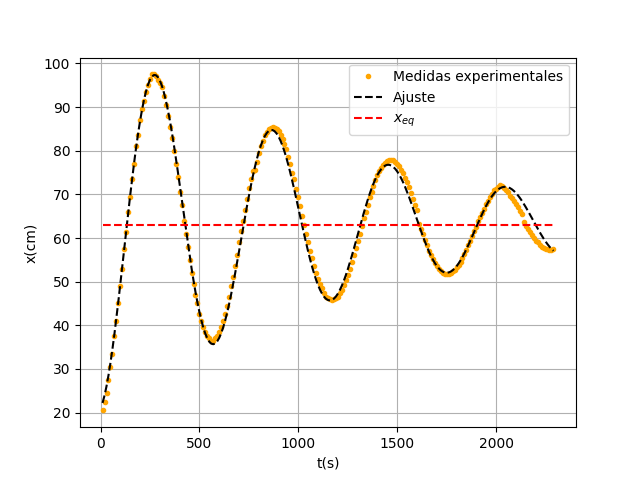
\includegraphics[width=0.95\linewidth]{Images/disposicion1.png}
        \subcaption{Oscilaciones con la disposición 1}
    \end{subfigure}
    \begin{subfigure}{0.49\textwidth}
        \centering
        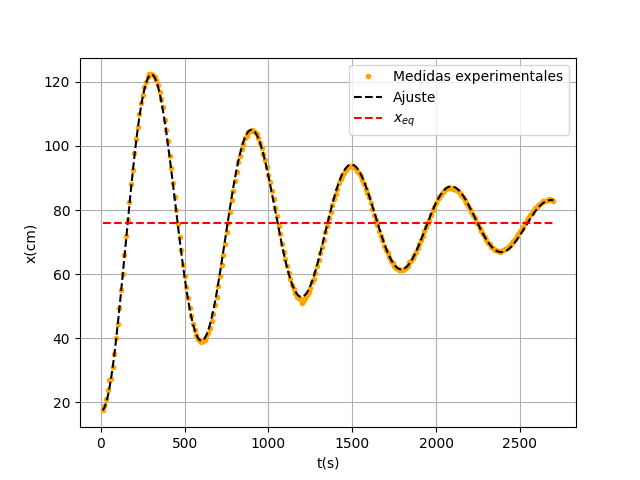
\includegraphics[width=0.95\linewidth]{Images/disposicion2.png}
        \subcaption{Oscilaciones con la disposición 2}
    \end{subfigure}
    \caption{Ajuste y medidas experimentales de $x(t)$}
\end{figure}

Los valores para los coeficientes obtenidos a partir del ajuste son:

\begin{table}[h!]
    \centering
    \begin{tabular}{|c|c|c|c|c|c|}
        \hline
        Parámetro & $x_{eq}(cm)$ & $A(cm)$ & $\gamma(s^{-1})$ & $\omega_1(s^{-1})$ & $\phi(rad)$ \\ \hline
        Disposición 1 & $63,01(64)$ &$-42,(59)$ & $7,738036(55) \cdot 10^{-4}$ &$0,01064022(75)$ & $0,1568(20)$\\ \hline
        Disposición 2 &$75,93(68)$ & $-58,(88)$ & $7,81985(30)\cdot 10^{-4}$ &$1.053690(30)\cdot 10^{-2}$ & $-6,3949(43)$\\ \hline
    \end{tabular}
\end{table}

Los valores que realmente nos interesan de este ajuste son la posición de equilibrio $x_{eq}$ que se da cuando la oscilación sea inapreciable y la frecuencia de oscilación $\omega_1$, que nos permite obtener el período $T$:

\begin{equation}
    T = \frac{2\pi}{\omega_1} \Rightarrow s(T) = \frac{2\pi s(\omega_1)}{\omega_1^2} \Rightarrow \left\{ \begin{array}{l}
        T_1 = 590.5123090 \pm 8,2 \cdot 10^{-6} \; s\\
        T_2 = 596.3028522 \pm 8,3 \cdot 10^{-6} \; s
    \end{array}\right.
\end{equation}

El valor final del periodo será la media ponderada de los valores obtenidos para las dos disposiciones:

\begin{equation}
    T = 593.3510825 \pm 5,8 \cdot 10^{-6} \; s
\end{equation}

\newpage

A partir de nuestro ajuste podemos obtener también las curvas de error de los dos conjuntos de medidas, que representa lo que se ajusta la curva teórica a los datos experimentales. Para ello vamos a representar el error de $x$ con su incertidumbre en función del tiempo. Definimos el error de $x$ como:

\begin{equation}
    x_{err} = |x_{exp}-x_{T}|
\end{equation}

\begin{figure}[h!]
    \centering
    \begin{subfigure}{0.49\textwidth}
        \centering
        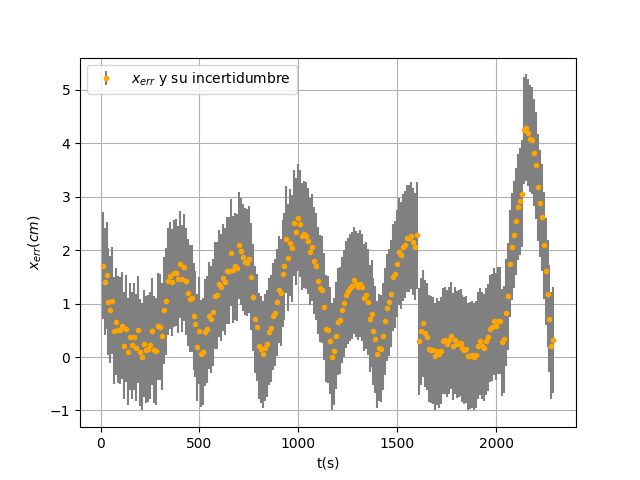
\includegraphics[width=0.95\linewidth]{Images/error1.png}
        \subcaption{Error de las medidas en la disposición 1}
    \end{subfigure}
    \begin{subfigure}{0.49\textwidth}
        \centering
        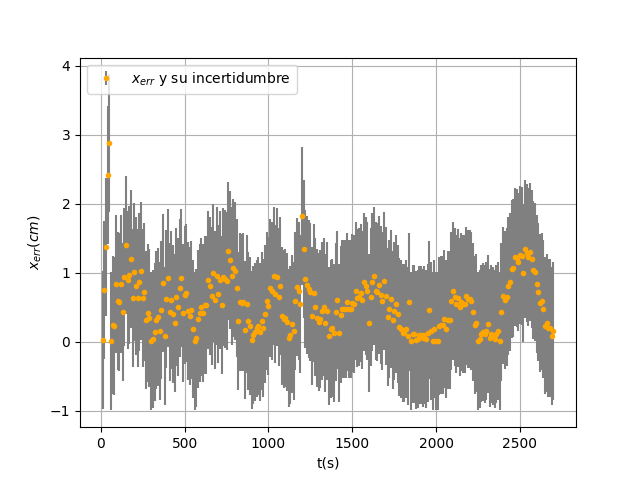
\includegraphics[width=0.95\linewidth]{Images/error2.png}
        \subcaption{Error de las medidas en la disposición 2}
    \end{subfigure}
    \caption{Representación de $x_{err}$}
\end{figure}

La representación gráfica del error nos muestra un patrón bastante claro en la forma en que este se ditribuye. Podemos ver que $x_{err}$ sigue una clara tendencia oscilatoria, adaptándose a una función sinusoidal, algo que cabría esperar teniendo en cuenta el carácter sinusoidal de la función $x(t)$ de la que proviene ese error.

\par Otro de los parámetros a estimar es la distancia media $b$ que hay entre las masas $M$ y $m$. Para ello vamos a emplear la relación entre los torques en la situación de equilibrio, donde la fuerza gravitatoria y la fuerza recuperadora de la balanza son iguales. La relación que obtenemos es:

\begin{equation}
    \left. \begin{array}{l}
        N_{eq}= 2\frac{G_NMm}{b^2}d\\
        N_{eq} = \frac{2\pi^2m\Delta x}{T^2L}d^2
    \end{array} \right\} \Rightarrow b = \sqrt{\frac{G_NMT^2L}{\Delta x\pi^2d}}
    \label{b}
\end{equation}


Donde $L$ es la distancia entre el foco emisor de luz y la pared, $d$ es la distancia entre el eje de giro y el centro de masas de la masa $m$, valor que tenemos como dato antes de empezar y $\Delta x=|x_{eq}^{II}-x_{eq}^{I}|$. Para medir $L$ tomamos datos de las longitudes de las baldosas de la clase de un extremo a otro de la pared para saber la longitud total de la clase y luego le restamos la distancia entre el espejo y la pared donde este estaba fijado. La expresión obtenida es la siguiente:

\begin{equation}
    L = L_1+L_2+nL_3-L_A
    \label{L}
\end{equation}

\newpage

Donde los términos $L_i$ se indentifican con:

\begin{itemize}
    \item $L_1=15 \pm 0,1 \;cm$ Es la baldosa cortada de un extremo
    \item $L_2=22\pm 0,1 \;cm$ Es la baldosa cortada del otro extremo
    \item $nL=560\pm 1,4 \;cm, \;n=14$ Es la longitud de las baldosas intermedias.
    \item $L_A=17,1\pm 0,15 \;cm$ Es la distancia entre el espejo y la pared, que se compone de la longitud de la barra y la mitad de la longitud de la caja. 
\end{itemize}

El valor obtenido a partir de la Ec.\ref{L} es:

\begin{equation}
    L=579,9 \pm 3,1 \;cm
\end{equation}

Una vez calculado este término ya podemos proceder a hacer una estimación del parámetro $b$ con la Ec.\ref{b}. El valor obtenido, con su incertidumbre es:

\begin{equation}
    b = 0,0566 \pm 0,0044 \;m
\end{equation}

Ahora ya podemos calcular el valor de la constante gravitacional $G_N$ empleando la siguiente fórmula:

\begin{equation}
    G_N = \frac{\pi^2b^2d}{ML}\frac{\Delta x}{T^2(1-\beta)}
    \label{Gn}
\end{equation}

Donde el factor $1/(1-\beta)$ es la corrección debido al torque de la otra esfera, el valor de $\beta$ sigue la siguiente expresión:

\begin{equation}
    \beta = \frac{b^3}{(b^2+4d^2)^{3/2}}
\end{equation}

El valor obtenido para la constante $G_N$ es de:

\begin{equation}
    G_N = 7,575 \cdot 10^{-11} \pm 9,3\cdot 10^{-13} N \cdot M^2 \cdot kg^2
\end{equation}

El valor obtenido para $G_N$ se acerca bastante a la realidad ($6,67\cdot 10^{-11}N\cdot m^2 \cdot kg^{-2}$) y el rango de incertidumbre es lo suficientemente pequeño para considerar esta medida válida. A continuación desglosaremos la incertidumbre de $G_N$, analizando todos los términos que forman parte de ella.

\subsection{Análisis de $s(G_N)$}

A partir de la Ec.\ref{Gn} podemos deducir que la constante gravitacional es función de los términos $G_N=G_N(b,d,\Delta x,M,L,T,\beta)$ siendo el resto de términos constantes. Por tanto su incertidumbre se obtiene por propagación con la siguiente expresión:

\begin{equation}
    \sqrt{u_b^2+u_d^2+u_{\Delta x}^2+u_M^2+u_L^2+u_T^2+u_\beta^2}
\end{equation}

Donde $u_{i}$ es la aportación de cada variable a la incertidumbre y tiene la siguiente expresión:

\begin{equation}
    u(x_i) = s(x_i)\left(\frac{\partial G_N}{\partial x_i}\right)
\end{equation}

\newpage

En la siguiente tabla podemos ver el aporte a la incertidumbre ($u(x_i)$) de cada variable:

\begin{table}[h!]
    \centering
    \begin{tabular}{|c|c|c|c|c|c|c|c|}
        \hline
        $x_i$ & $u_b$ & $u_{\Delta x}$ & $u_M$ & $u_L$ & $u_T$ & $u_{\beta}$   \\ \hline
        $u(x_i)$ & $6,6\cdot 10^{-13}$ & $1,1\cdot 10^{-13}$ & $5,1 \cdot 10^{-13}$ &
        $4,0\cdot10^{-13}$ & $1,5\cdot 10^{-18}$ & $1,0\cdot 10^{-13}$ \\ \hline
    \end{tabular}
    \caption{Análisis del aporte a la incertidumbre $s(G_N)$ de cada variable}
\end{table}

A partir de esta tabla podemos ver que las variables que aportan más incertidumbre son $b$, $M$ y $L$.En estas dos últimas podemos entender fácilmente la alta incertidumbre ya que son medidas directas, para mejorar su incertidumbre habría que aumentar la precisión experimental. Por otro lado, el gran aporte de $b$ a la incertidumbre se debe a que, aunque es una medida indirecta, se obtiene a partir de $M$ y $L$, por lo que es normal que tenga una incertidumbre razonablemente alta.

\subsection{Obtención de la constante de torsión $k$}

Por último, vamos a calcular el valor de la constante de torsión de la balanza a partir de la siguiente expresión:

\begin{equation}
    k = \frac{8\pi^2m}{T^2}d^2
    \label{k}
\end{equation}

Donde $m$ representa el valor de las masas que se encuentran dentro de la balanza, a priori desconocido. Para calcularlo vamos a emplear el resto de datos que tenemos sobre las bolas, tenemos sus radios y la masa $M$ de las bolas grandes. La magnitud que relaciona todos estos datos es la densidad de las bolas, que vamos a suponer aproximadamente igual ya que ambas son de plomo.

\begin{equation}
    \rho = \frac{m}{V} = \frac{m}{\frac{4}{3}\pi r^3}
\end{equation}

Sustituyendo los valores de la masa grande $M=1500 \;g$ y $r_{M}=3,158\;cm$ obtenemos el siguiente valor para la densidad:

\begin{equation}
    \rho = 11,370 \pm 0.076 \;g\cdot cm^{-3}
\end{equation}

A partir de la densidad ya podemos calcular el valor de la masa $m$:

\begin{equation}
    m = \rho \cdot V_m = \frac{4}{3}\rho \pi r_m^3 = 26,26 \pm 0,17 \;g
\end{equation}

Con este valor ya podemos calcular la constante de torsión sustituyendo en la Ec.\ref{k} todos los datos:

\begin{equation}
    k = 1,4723 \cdot 10^{-8} \pm 9,8 \cdot 10^{-11} \;N\cdot m
\end{equation}

\section{Conclusiones}

Para finalizar cabe destacar el buen valor obtenido para la constante gravitacional ($G_N = 7,575 \cdot 10^{-11}\;N\cdot m^2 \cdot kg^{-2}$), que era el objetivo principal del experimento, obteniendo un valor que se encuentra en el mismo orden de magnitud y muy próximo al real. Esto es algo a destacar ya que la balanza de torsión es un instrumento de medida especialmente sensible a perturbaciones externas, algo que se podría esperar que sucediera al estar llevándose a cabo otras prácticas a nuestro alrededor.



\end{document}